\documentclass{llncs}
\usepackage{times}
\usepackage{gensymb}
\usepackage{parskip}
\usepackage{graphicx}
\usepackage{float}
\usepackage[hyphens]{url}
\usepackage{hyperref}
\usepackage{array}
\usepackage{multirow}
\usepackage{caption} 
\captionsetup[table]{skip=10pt}
\hypersetup{breaklinks=true}
\urlstyle{same}
\graphicspath{ {Figures/} }   
\begin{document}

%New Technology to Connect Internet: Google Balloon and Facebook Drone

	%Top Matter
	\title{New Technologies to Connect Internet: Google Balloon and Facebook Drone }
	
           \author{Vaibhav Kasturia\inst{1} \and Enhuan Dong\inst{2}}	
	
           \institute{L3S Research Center, Leibniz Universit\"{a}t Hannover, 30167 Hannover, Germany
           \\\email{kasturia@l3s.de} 
           \and 
           Institute of Computer Science, Georg-August-Universit\"{a}t G\"{o}ttingen, 37073 G\"{o}ttingen, Germany\\
	\email{edong@gwdg.de}
	}	
	
	\maketitle
	
	\tolerance=1
           \emergencystretch=\maxdimen
           \hyphenpenalty=10000
           \hbadness=10000

	\begin{abstract}
	\noindent Google Balloon and Facebook Drone are futuristic and state-of-the-art projects by Google and 
	Facebook with the aim of connecting the world by providing internet access to people living in areas
	where it would be infeasible to provide internet using current infrastructure and methods. Current 
	estimates show that only one-third of the earth's population has internet access and that people are 
	mainly dependent on the Internet Service Providers (ISPs) for internet access. Facebook Drone and Google 
	Balloon aim to change that by providing coverage everywhere, specially in regions where fixed permanent  
	infrastructure is impossible to build and where using satellite communication would prove to be too expensive. 
	This paper shows how these new technologies are economically more feasible and highlights the design behind 
	these technologies. It further talks about the new invisible laser technology used to provide 
	communication links by both these projects. Based on the prototype designs and test flights conducted so far, 
	it draws a comparison between the two projects and highlights the potential challenges to be overcome in 
	order to be able to bring these technologies to people in the future. 
	    	
	\end{abstract}
	
	\section{Introduction}
	The growth of the Internet has been tremendous in the recent years. Even though the number of 
	Internet users has been increasing, a study done by Facebook in 2014 estimated that currently only one-third of the earth's 
	population has access to the Internet. Today, 80 to 90 percent of the world's population lives in areas
	which have 2G or 3G network coverage. Despite this, the Internet access being available to just 33 per cent of 
	the people in the world shows that most of the people cannot access the Internet primarily due to economic 
	challenges. For the remaining 10 to 20 percent people, however, the challenges posed to accessing the Internet 
	are both infrastructure and economic challenges. The aim of Google Balloon and Facebook Drone is to exactly 
	capture the market provided by those 10 to 20 percent which live in areas where providing infrastructure for 
	Internet Access by the current methods is either infeasible due to the population density being very less or 
	because the terrain or the cost does not permit building a permanent infrastructure.   
	According to the estimates by Facebook, providing Internet to the people in these areas could have the potential to
	create 140 million job opportunities and could uplift 160 million poor people out of poverty\cite{facebookdrone}. 
	
	\section{Motivation behind these Technologies}
	
    \indent The motivation behind using technologies like Google Balloon and Facebook Drone over current methods of 
    communication such as Satellite Communication or building fixed infrastructure such as radio towers are 
    numerous. One such major motivation is the Law of Signal Power Attenuation, a basic law of Physics according 
    to which the radio power of a signal weakens as a square of distance. This basically means that if you have a 
    source emitting radio waves then if you move a distance of 4 times the current distance, the power of the signal 
    you would receive would be 16 times weaker than the power of the signal you would receive at the current distance.
    Figure \ref{fig:signal_power_attenuation} better illustrates this problem. 
    
    \begin{figure}[ht]
	\centering
	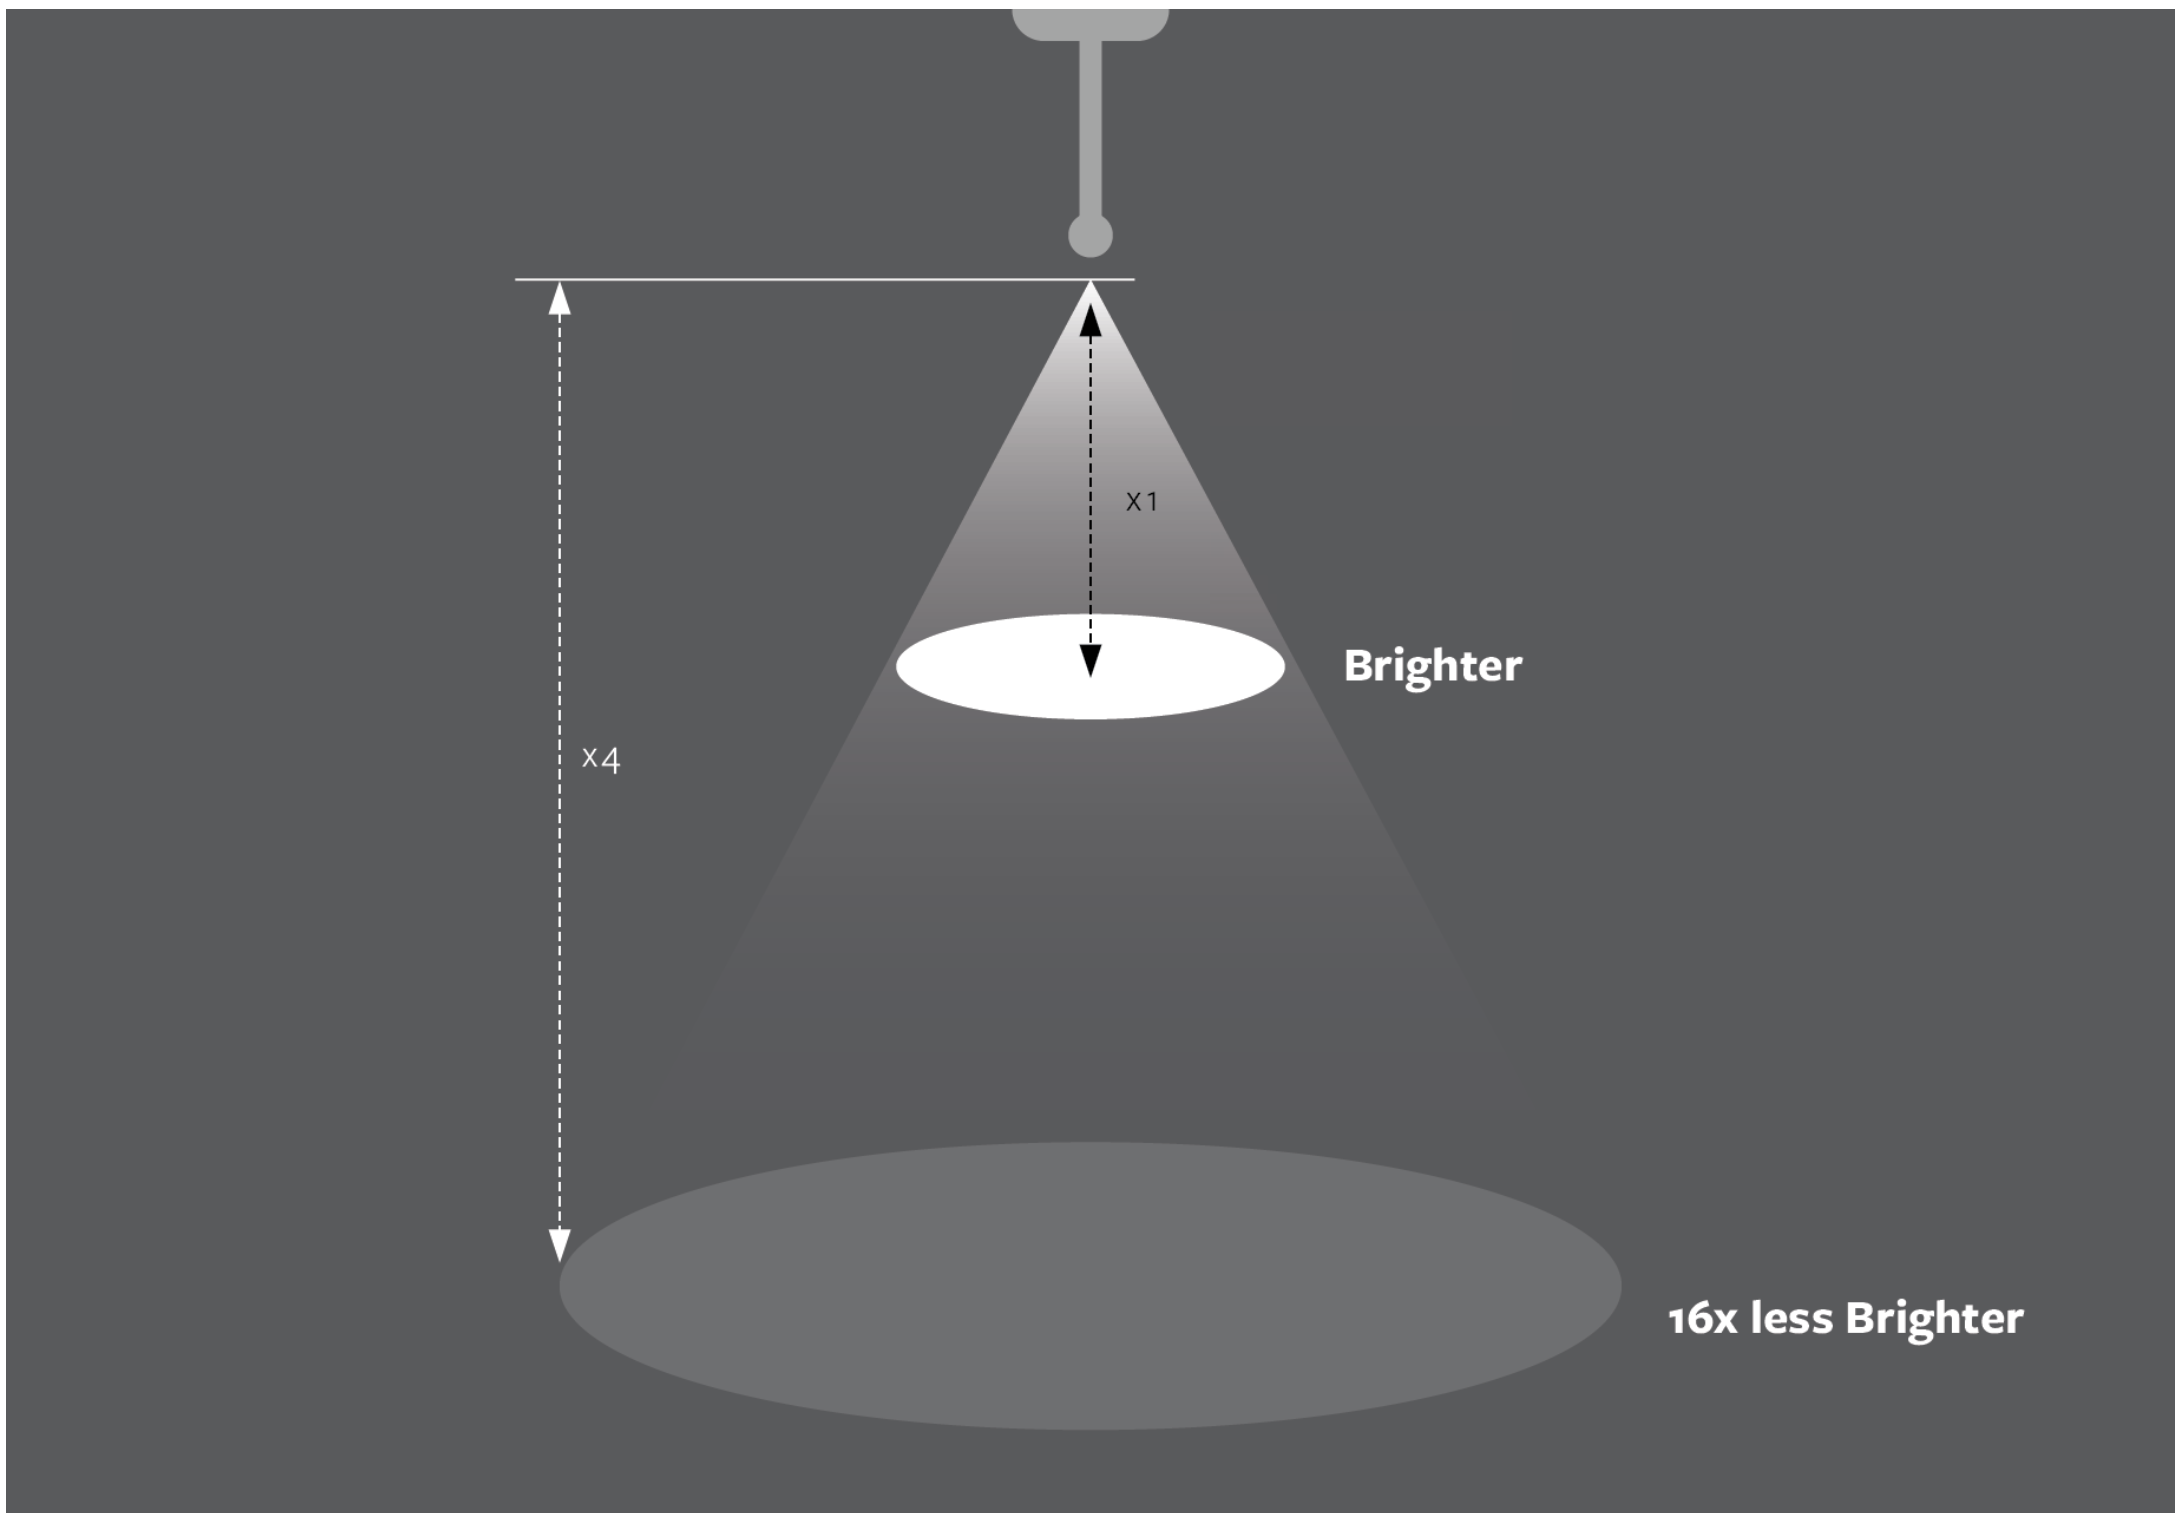
\includegraphics[width=0.95\textwidth]{fig1}
	\caption{Physics of Electromagnetic Propagation}
	\label{fig:signal_power_attenuation}
    \end{figure}
    
    Figure \ref{fig:platforms_altitudes} shows the connectivity density for platforms at
    different altitudes. Due to the Signal Power Attenuation problem, if satellites were to be used for providing 
    Internet Access, we would be either required to build huge, solar powered satellites, the structures of which
    would turn out to be unstable or build nuclear-powered satellites which would be very expensive. Moreover, 
    satellites have a higher cost of deployment compared to Facebook Drone or Google Balloon. 
    
    \begin{figure}[H]
	\centering
	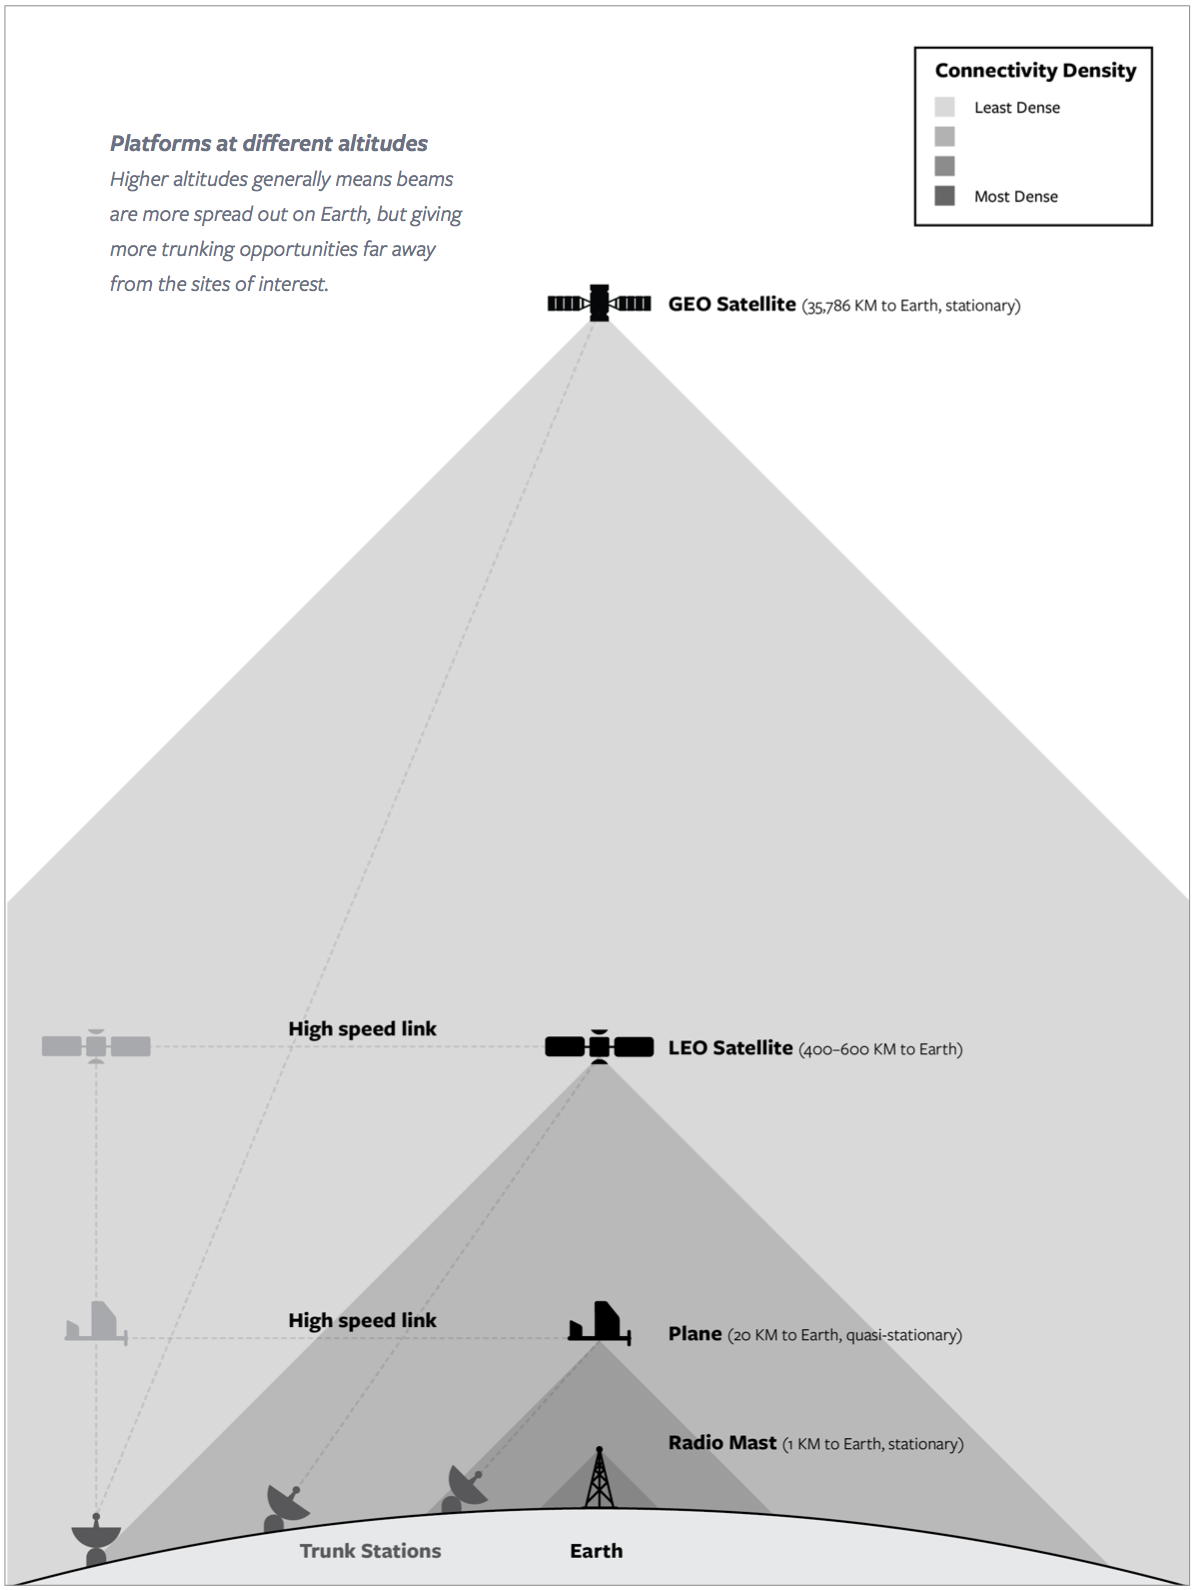
\includegraphics[width=0.9\textwidth]{fig2}
	\caption{Platforms at different altitudes}
	\label{fig:platforms_altitudes}
    \end{figure}
    
    Among satellites too, the cost of deployment for Low Earth Orbit(LEO) satellites is lesser when compared to Geosynchronous Earth 
    Orbit(GEO) satellites as LEO satellites are just situated at a distance of 400-600 km to the earth when compared
     to GEO satellites which are situated at a distance of 35,786 km to the earth, making LEO satellites more cheaper
     to deploy through rockets than GEO satellites. However, using LEO satellites has disadvantages such as these 
     satellites not being stationary due to the rotation of the earth around its axis requiring the building of a lot
     of ground stations to constantly track satellite movement. Further, in order to just cover 100 people per square
     km a constellation of LEO satellites would be required. GEO satellites have the advantage that they remain 
     stationary when taking into account to the rotation of the earth around its axis. Hence, they require lesser 
     number of ground stations than LEO satellites for monitoring. But the higher costs of deployment and even weaker 
     signals due to larger distance render them ineffective as well for communication in medium density population 
     areas. 
     
     A balloon or a drone forms the ideal solution to cater to people living in such medium density population areas. 
     They fly at a distance of 18 km to the earth, just above the unregulated airspace (according to United States 
     norms, the unregulated airspace starts at a distance of 18 km from the earth's surface\cite{us_airspace}). Less stronger winds at
     this height allow for more precise location control and allow for these unmanned aerial objects to stay aloft 
     with lower energy consumption. These structures can be powered by solar energy. Further, they are cheap to build
     and re-usable. Even in war zones or in places where natural calamities occur frequently, such structures are 
     ellective as radio towers or any ground infrastructure are always prone to destruction whereas these are not. 
     Thereby, their usage seems to be the most effective in providing Internet access in such areas.     
	
\section{Google Balloon}
Google Balloon, called the Project Loon\footnote{\url{https://x.company/loon/}}, 
is a research and development project of Google X\footnote{\url{https://x.company/}} and has the mission of
providing internet access to people living in remote and rural areas. The project uses high-altitude balloons placed in 
the stratosphere to create an aerial wireless network with up to 4G LTE Speeds. The balloons are made up of polyethylene, 
launched using an auto-launcher crane and are equipped with a flight capsule, transceivers, solar panels and parachute. The 
balloons move in the stratosphere and are navigated using the air movement of the different wind layers of the stratosphere.
Figure \ref{fig:balloon_coverage} describes how network of balloons in Project Loon provides coverage. Google has flown over 19 million km of test flights since the project began. The subsections describe all the aspects of 
balloon in detail.  	

\begin{figure}[ht]
	\centering
	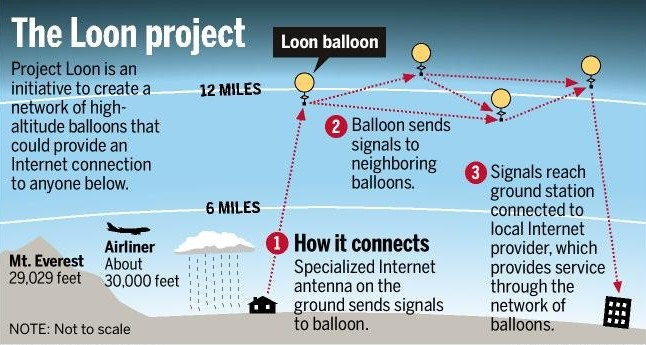
\includegraphics[width=0.95\textwidth]{fig3}
	\caption{Providing Coverage using Balloons}
	\label{fig:balloon_coverage}
    \end{figure}
	
\subsection{Design}
The balloons are made up of Polyethylene Sheets in order to reduce costs. Google used a special atmospheric chamber designed by the National 
Aeronautics and Space Administration(NASA)\footnote{\url{https://www.nasa.gov/}} to simulate the atmospheric conditions. The balloons are 
subjected to pressure, temperature and winds similar to those conditions found at that height and then strain on the balloons is checked with 
inflation and deflation to see when the balloon bursts. Before these simulations were conducted balloons used to keep bursting in the 
atmosphere after just 3 days. Now with the improved testing balloons can survive wind speeds of up to 100 km per hour, temperatures of up to -90\degree{C} and UV Radiation. The balloons now have an improved lifetime of a 100 days. 	
	
	\subsection{Launching}
	In the initial runs, the ground air used to affect deployment of the balloons by changing their trajectory so Google 
	designed an auto-launcher crane for launching the balloons automatically and to tackle the affect of ground air. 
	This auto-launcher crane has been nicknamed ``Chicken Little".
	Side Panels on three sides of the crane provide protection against ground air and the balloons are launched in a 
	leeward fashion to minimize the effect of ground air from the front. The auto-launcher crane has a capacity to 
	launch one balloon every 30 minutes.
	
	\subsection{Equipment}
	Each balloon is equipped with a Flight Capsule, Transceivers, Solar Panels and Parachute. Flight Capsule 
	acts as 
	the brain of the balloon and collects all its flight data. Transceivers are used for ground communication 
	and for 
	inter-communication between the balloons. Solar Panels gather solar energy used for powering the balloon. 
	The 
	Parachute is used to bring the balloon down after it has completed its life-time for re-use or its 
	automatically
	deployed in case of emergencies like bursting of the balloon. 
	
	\subsection{Navigation}
	The movement of the balloon is in the Stratosphere. In the stratosphere each wind layer moves in a different 
	direction. To move the balloon left or right, the balloon just needs to be moved up or down to be placed in 
	the appropriate layer. After that the balloon will move in the direction of the wind layer. Google gets real-time data for the weather 
	conditions and
	the wind speed and direction in the different wind layers from the National Oceanic and Atmospheric 
	Administration (NOAA)\footnote{\url{http://www.noaa.gov/}}. A lot of decision making algorithms and navigational models are used to 
	determine
	correct placement of the balloon.   
	
	\subsection{Test Flights}
	Unofficial development of the Google Loon project started in 2011 under Google X, a semi-secret
	research facility that Google uses for research on its futuristic projects. A series of test flights
	was at that time conducted in California's Central Valley\cite{google_balloon_x}. 
	
	The project was officially announced by Google in 2013. On 16 June 2013, Google conducted a series
	of test flights from the Tekapo area of South Island in New Zealand\cite{google_balloon_x}. In coordination with the Civil
	Aviation authority, Google launched around 30 balloons and the connection was tested by around
	50 Users from in and around the Canterbury Region and Christchurch.      
	
	In May-June 2014, Google marked its very first LTE experiment and launch near the equator when it
	tested its Balloons in Piau\'{i}, Brazil\cite{google_balloon_brazil} and in the same year it also partnered with France's Centre 
	national d'\'etudes spatiales (CNES)\cite{google_balloon_france} on the project. Google has since increased its record streak 
	for an unmanned balloon from 50 days in February 2014 to 130 days in November 2014 and the latest
	one being 190 days in March 2015\cite{google_balloon_record}. 
	
	In 2015, Google signed agreements with two countries, Sri Lanka and Indonesia, to bring its Project 
	Loon there. Sri Lankan officials of the Information and Communication Technology Agency (ICTA) of Sri 
	Lanka signed agreements with Google on 28 July 2015\cite{google_balloon_srilanka} to launch the technology on a mass scale which made Sri Lanka the 
	second country in the world in March 2016 to get full coverage of Internet using LTE. In Indonesia, 
	with the hopes of providing internet access and connecting the country's 17000 islands, Google partnered with  XL Axiata, Indosat and Telkomsel on 29 October 2015\cite{google_balloon_indonesia}. 
	
	As of 2016, Google tested its auto-launcher crane, nick-named ``Chicken Little", at a former naval station Roosevelt Roads located in Ceiba, Puerto Rico\cite{google_balloon_autolauncher}. It also has conducted test flights in Canada as on 5 September 2016, a balloon was spotted over Newfoundland and Labrador, Canada. Google has future plans of sending up to 300 balloons at 40th parallel south around the world and these balloons would provide coverage to Australia, Argentina, Chile and New Zealand.    	
	  
	
	\section{Facebook Drone}
	Facebook solar-powered drone, codenamed the ``Aquila"\cite{drone_zuckerberg}, has an aim similar to that of Google Loon of 
	providing internet access to the people living in the rural and remote areas using a series of drones 
	instead of a constellation of balloons. Each drone is made up of composite carbon fibre, would be powered using solar energy, flies at low 
	speeds to stay aloft for as long as possible with minimum energy and is able to land automatically. Batteries account for most of the load 
	of the drone and the drone is expected
	to fly at an altitude of 60,000 to 90,000 ft. Facebook has till date successfully conducted one test flight of a prototype of its 
	drone. Figure \ref{fig:facebook_aquila} illustrates the design of the Aquila Drone. The highlights of all the aspects of the drone are 
	mentioned in the	subsections below.     
	
	\begin{figure}[H]
	\centering
	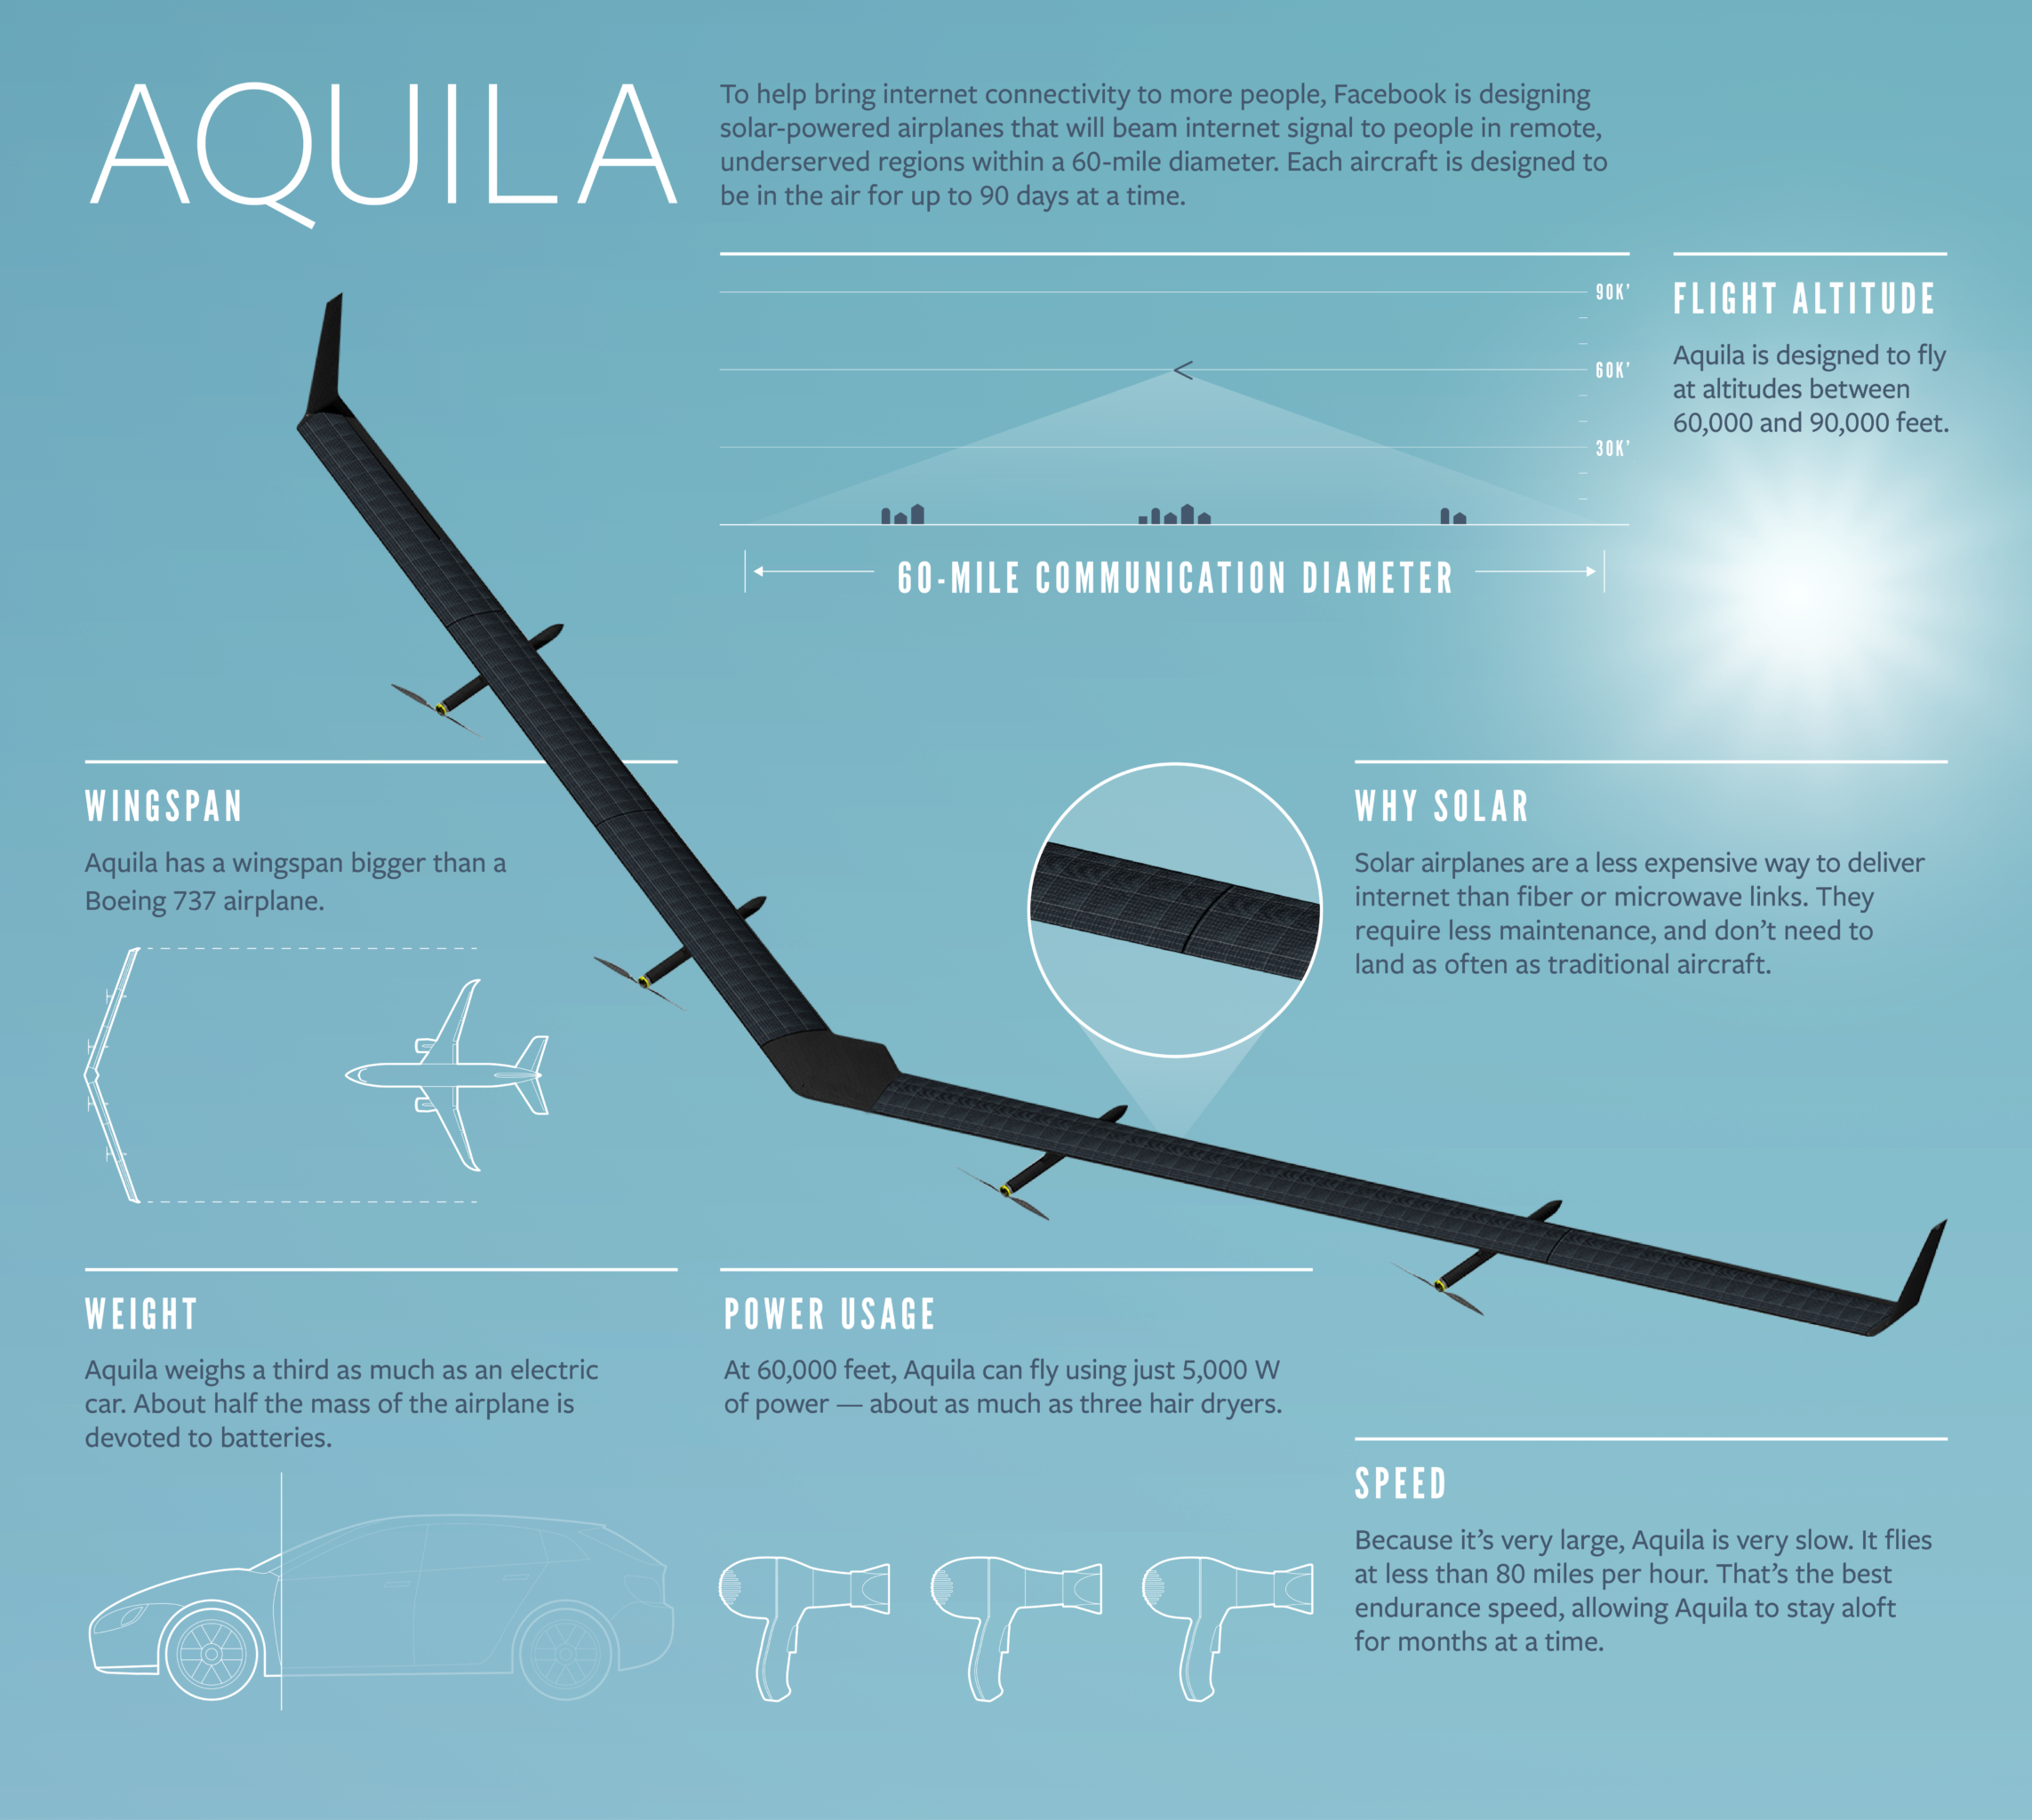
\includegraphics[width=1.0\textwidth]{fig4}
	\caption{Facebook Drone Aquila}
	\label{fig:facebook_aquila}
    \end{figure}
    
                \subsection{Weight}
	The Aquila drone has to have as less weight as possible to able to stay in the air as long as possible. The drone weighs less than 1000 
	pounds or 400 kilograms due to the whole body of the drone being made up of composite carbon fibre. The Facebook team is continually 
	investigating ways to make the drone even more lighter. It weighs just one-fifth of the popular Reaper Drone\footnote{\url{https://en.wikipedia.org/wiki/General_Atomics_MQ-9_Reaper}} used by the United States in 
	Afghanistan since 2006. The drone has a wingspan of 141 feet, 28 feet larger than the 113 feet wingspan of a Boeing 737.
	
	
	\subsection{Power}
           The drone once deployed would be powered by solar charged batteries that would get charged by the energy of the sun during the day. When it is dark, the energy collected would be used to power its propellers, avionics, communications payload and light and heating systems. The drone would be flying at a higher altitude at more speed during the day and will stoop down to a lower altitude and fly at lesser speed during the night. At cruising altitude the drone is expected to use 5000 W of power which is much the same as the power consumption of three hairdryers. 
           
           \subsection{Speed}
           Commercial flyers usually travel at a very high speed because these flights are used as a means of transport. The motive behind the drone being to stay in the air as long as possible, it is rather slow. The drone flies at a speed of 20 mph. The drone attains a maximum speed of 80 mph at higher altitudes due to the air being thinner at higher altitudes.
           
           \subsection{Control}
           The drone has been designed to mostly be self-sufficient. It has been designed to take off and land automatically as software is able to land the drone in a location more precisely than any human being is able to. The altitude, heading and airspeed is however controlled and monitored by a ground crew consisting of a dozen pilots, technicians and engineers through a software. The software also gives the ground crew the possibility to send the drone on a GPS based route.
           
           \subsection{Load}
           High-energy batteries account for almost half of the weight of Aquila drone. This load is quite huge for flexible wings made up of carbon fibre. Facebook currently uses computer models to predict deformation in the drone's shape under load. A better idea of deformation during flight would be obtained during test flights. 

           \subsection{Altitude}
           	Air at higher altitudes is colder and less denser as compared to air at lower altitudes which is warmer and much denser. The power consumption and impact of the altitudes on solar panel performance, latitude range, seasonal performance and battery size is currently under investigation by the Facebook team.
	
	
	\subsection{Test Flights}
	Facebook has held numerous attempts to test prototype versions of the Aquila Drone. Early on in 2015, they had attempted to launch the drone with a hot-air balloon but had failed to do so. They also planned a test flight for the drone in October 2015, but it had to be cancelled two times due to turbulence by the El Ni\~{n}o storms\cite{drone_test_flights}. 
	
	Facebook finally successfully tested a prototype version of the Aquila Drone on June 28, 2016 from an aviation testing facility in Yuma, 
	Arizona\cite{drone_test_flights}. The prototype version of the drone was powered by lithium ion batteries, much like those which are used 
	in mobile phones instead of solar panels as would be used in the final version. The Facebook team working on the drone had expected a 
	flight time of 30 minutes. The prototype version, however, exceeded this limit and after take off stayed in the air for nearly 90 minutes. 
	The final version of the drone is expected to stay in the air for nearly three months at a time. The team flew the prototype version at an 
	altitude of just 2000 ft, much less than the altitude of 60,000 to 90,000 ft planned for the final version. And unlike the 5000 W of 
	energy the final version of the drone is expected to consume, the prototype version just consumed 2000 W of energy. During the test 
	flight, he prototype version suffered what the engineering team described as a ``structural failure" which caused serious damage to the 
	drone shortly before landing to an extent that the National Transport Safety Board (NTSB) which investigated the incident termed it as an 
	``accident" meaning that the damage makes the prototype no longer capable of flying\cite{drone_failure}. No other details about the accident were revealed by 
	either NTSB or Facebook.   
	
	\section{Free Space Optics (FSO)}
	Free Space Optics(FSO)\cite{facebookdrone} is a technology which is used by both Facebook Balloon and Google Drone. FSO are 
	invisible 
	IR laser beams. They have a very high bandwidth and capacity, at par with fibre optic cables. The expected 
	data 
	transfer rate is about 10 Gigabits per second which is about ten times faster than the existing systems. 
	Since 
	laser beams 	are focussed, they use less power than microwaves. They are so precise that they can 
	accurately hit a 
	coin from ten miles away. Moreover, the FSO Spectrum remains unregulated at present whereas the microwave 
	spectrum 
	is already regulated. The thing that remains to be seen in future whether this technology will also be regulated 
	by 
	countries.    
	
    \section{Comparison}
    	In this section, we compare the different aspects of both Facebook Drone and Google Balloon. Table \ref{tab:comparison}
    	draws a comparison between the different features of both Facebook Drone and Google Balloon. 	In terms of 
    	cost, it is safe to say that the costs of manufacturing and deployment of the Facebook Drone are 
    	significantly more than that of Google Balloon, which uses polyethylene sheets for manufacturing the balloons
    	and uses the auto-launcher crane which is a much cheaper method for deployment. 
    	
    	Navigation, however, turns out to be better for Facebook Drone as compared to the Google Balloon as the 
    	drone can be more precisely controlled. Google Balloon, on the other hand is more difficult to control as 
    	constantly real-time data from the National Oceanic and Atmospheric Administration (NOAA) regarding weather 
    	conditions, temperature and wind speed in the different wind layers is required. Then complex decision making 
    	algorithms and navigation models need to be used to determine the appropriate wind layer in which the 
    	balloon is to be placed. The movement of the cluster of balloons need to be synchronized as well in order 
    	to provide continuous connection to the user at the ground. 
    	
    	In terms of endurance, the current world record held by a drone has been two weeks. This drone was owned by 
    	Ascenta, a company was later acquired by Facebook. According to Facebook, once completed, the final version 
    	of the drone is expected to have a flight time of 90 continuous days without the need for landing. The 
    	prototype version of the drone tested till now just had a flight
    	time of 90 minutes. Google Balloon, on the other hand has already achieved a 190 day flight record 
    	\cite{google_balloon_record}. Each balloon in its final version is expected to have a flight time of 100 days. According to 
    	Mark Zuckerberg, the Founder of Facebook, the drone in its final version would outweigh the Google Balloon in
    	the time the aerial vehicles stay in the air without landing. 
    	
    	Taking into account accidental risks, the risks of damage caused by the Facebook Drone crash would be more 
    	than the Google Balloon crash. Google Balloon has a parachute which deploys automatically in case the 
    	balloon bursts. Also, the damage caused would be lesser as the Google Balloon is made up of plastic sheet 
    	though it has other equipment also but the drone is made up completely of carbon fibre.           
	
	\begin{table}[h]
	\hskip-1.5cm
	\begin{tabular}{|c|l|l|}
    \hline
    \multicolumn{3}{|c|}{\textbf{Comparison}} \\
    \hline
    \multicolumn{1}{|c|}{\textbf{Aspect}} & \multicolumn{1}{c|}{\textbf{Facebook Aquila Drone}} & \multicolumn{1}{c|}{\textbf{Google Project Loon}} \\ \hline 
    Cost & - Greater Manufacturing and Deployment Costs & - Comparatively very cheap to manufacture and deploy \\ \hline
    \multirow{2}{*}{Navigation} & - Precise and Easier Location Control & - More Difficult \\
    &  & - Real Time Climate Data by NOAA Required \\ \hline
    \multirow{2}{*}{Endurance} & - 2 Weeks World Record\cite{drone_test_flights} & - 190 Days World Record\cite{google_balloon_record} \\
    & - 90 Days in final models & - 100 Days per Balloon \\ \hline
    \multirow{2}{*}{Accident Risks} & - No Emergency Deployment Measures & - Emergency Parachute Deployment \\
    & - Higher when compared to Google Balloon & - Lesser Risks and Damage when compared to Drone \\ \hline
    \end{tabular}
    \caption {Comparing the different aspects of Facebook Drone and Google Balloon}
    \label{tab:comparison}
    \end{table}
    
	\section{Future Challenges}
	Many challenges remain to be addressed for both Facebook Drone and Google Balloon. 
	For Facebook Drone, the  best method of deployment of the drone still needs to be decided. 
	Deployment still remains a major concern for Facebook Drone because putting a drone at the height of
	60000 to 90000 feet needs to be cost effective. Facebook has already tried deployment of the drone 
	with hot air balloons once in 2015 and failed. In the test flight of the prototype version in 
	June 2016 in Yuma, Arizona, they had used a plane for deployment but they flew the prototype version at the
	height
	of just 2000 ft\cite{drone_test_flights}. Facebook is still undecided on whether it would use a hot air-balloon or a plane for the 
	deployment of the final versions of the drone. 
	
	Another challenge for the Facebook Drone is building
	a version that can run without batteries. The prototype version built in 2016 ran on heavy batteries 
	made up of lithium ion. The final version of the drone is expected to be fully powered by solar 
	energy. Endurance is still a problem for Facebook Drone. The prototype version being made up of 
	lithium ion batteries was heavy and because of its weight just had a flight time of 90 minutes. 
	If Facebook expects it final version to outweigh the flight time of Google Balloon, which already has 
	made a record flight time of 190 days, then it needs to focus on building a lighter drone version 
	powered by solar energy. 
	
	Safety still remains a concern for both Facebook Drone and Google Balloon. 
	During the same test flight of the Facebook Drone as mentioned earlier, the drone suffered something
	which was described as a ``structural failure" that caused significant damage to the drone while 
	landing. If an accident were to happen in the final version then the risks and damages caused by the 
	drone could be significant. A similar incident happened when a Google Balloon crashed in the front 
	yard of a house in Chino Hills, a suburb in Los Angeles, California\cite{balloon_crash}. The Google Balloon was supposed
	to land in a designated area but crashed before reaching its intended destination. The risks and 
	damages from unmanned flying objects falling from the sky could be tremendous. 
	     
                Lastly, it remains to be seen how both Facebook and Google deal with local governments of countries 
                for the deployment of these technologies. An article by the Telegraph \cite{balloon_ban} reported that Google 
                Balloon may already face ban in India, one of its biggest potential markets, due to regulatory issues. 
                There were several issues pointed to Google by the Department of Telecommunications in India which 
                may prevent the Balloon getting a go ahead.
                Facebook also needs to look upon its handling with the governments across countries. Internet.org\footnote{\url{https://info.internet.org/en/}}, 
                an initiative by Facebook to provide free Internet Services was already banned in India\cite{internetorg_ban} with the 
                government citing net neutrality issues and the assumption that the only concern of Facebook being the huge revenues
                it stands to gain through advertisement on this platform as the main reasons for the ban.
               
	 \section{Conclusion}
	 Facebook Drone and Google Balloon are novel technologies that hold potential to connect millions
	 of people across the world. They are more cost-effective than Satellite Communication and ideal to 
	 connect people living in medium density areas and in places where building fixed infrastructure
	 is infeasible. They are several hindrances that need to be yet overcome. For example, the Weight, Cost 
	 and Endurance still pose a major challenge for Facebook Drone. Moreover, these technologies do not 
	 come without risks of accidents. Apart from technological issues, concerns regarding the airspace 
	 usage, radio spectrum and other issues need to be solved with Local Governments in order to 
	 be able bring these technologies to the people. If these concerns are not overcome, there might
	 be a ban across countries and this might make such technologies not foreseeable in the near future.   

\Urlmuskip=0mu plus 1mu\relax
\bibliographystyle{abbrv}
\bibliography{bib/drone_balloon.bib}
	
\end{document}